\section{投影梯度法（PGD）}
\label{sec:feas-pgd}

梯度步把点带出可行集合，能不能走完再拉回来，并且仍然保留梯度下降的保证？本节回答这个问题：先算投影，再说明残差应该怎样定义，最后证明下降和收敛。

\paragraph{主要思想}
回想第~\ref{chap:smooth-foundations}章的二次上界。在当前点$\bm{x}$，无约束的梯度步是在全空间最小化上界模型。现在只在$\bm{C}$上最小化同一个模型：
\[
 \bm{x}^{+}=\argmin_{\bm{y}\in\bm{C}}\Bigl\{f(\bm{x})+\langle\nabla f(\bm{x}),\bm{y}-\bm{x}\rangle+\frac{1}{2\alpha}\lVert\bm{y}-\bm{x}\rVert_2^2\Bigr\}.
\]

把花括号里关于$\bm{y}$的部分配方，常数项不影响最小点，得到
\[
 \bm{x}^{+}=\argmin_{\bm{y}\in\bm{C}}\frac{1}{2\alpha}\bigl\lVert\bm{y}-\bigl(\bm{x}-\alpha\nabla f(\bm{x})\bigr)\bigr\rVert_2^2.
\]
这正是求$\bm{C}$中离梯度步终点最近的点。

记$\bm{C}$上的欧氏投影为
\begin{equation}
 P_{\bm{C}}(\bm{z})=\argmin_{\bm{y}\in\bm{C}}\lVert\bm{y}-\bm{z}\rVert_2,
 \label{eq:feas-projection}
\end{equation}
\term{投影梯度法}（projected gradient descent，PGD）的迭代就是
\begin{equation}
 \bm{x}^{(t+1)}=P_{\bm{C}}\bigl(\bm{x}^{(t)}-\alpha^{(t)}\bm{g}^{(t)}\bigr).
 \label{eq:feas-pgd}
\end{equation}

第~\ref{chap:nonsmooth-composite-optimization}章把投影看作约束指标函数的邻近映射，这里复述要用到的三条结论。对非空闭凸集，投影存在且唯一；$\bm{p}=P_{\bm{C}}(\bm{z})$当且仅当$\bm{p}\in\bm{C}$且
\begin{equation}
 \langle\bm{z}-\bm{p},\bm{y}-\bm{p}\rangle\leq0,\quad\forall\bm{y}\in\bm{C};
 \label{eq:feas-projection-vi}
\end{equation}
投影不会拉大距离，也就是
\begin{equation}
 \lVert P_{\bm{C}}(\bm{u})-P_{\bm{C}}(\bm{v})\rVert_2\leq\lVert\bm{u}-\bm{v}\rVert_2.
 \label{eq:feas-nonexpansive}
\end{equation}

式~\eqref{eq:feas-projection-vi}有直观的几何含义：从$\bm{p}$看，$\bm{z}$和集合中任何一点的夹角都不小于直角。就像站在池塘边离某棵树最近的位置，整个池塘都在你身后的半边。

\subsection{投影计算}
\label{sec:feas-pgd-projection}

式~\eqref{eq:feas-pgd}的数学形式对所有闭凸集相同，能不能算则要看集合。本小节算出两个最常用的投影，并把预算例走几步。

\paragraph{盒约束}
设$\bm{C}=\{\bm{x}:\bm{l}\leq\bm{x}\leq\bm{u}\}$。目标$\sum_i(y_i-z_i)^2$和约束都按坐标分离，所以每个坐标单独处理：
\begin{equation}
 P_{\bm{C}}(\bm{z})_i=\min\bigl\{u_i,\max\{l_i,z_i\}\bigr\}.
 \label{eq:feas-box-projection}
\end{equation}
例如$\bm{C}=[0,1]^2$时，$(1.4,-0.3)$的投影是$(1,0)$。计算量是$O(n)$。

\paragraph{单纯形}
设$\bm{\Delta}$是$n$维概率单纯形：
\begin{equation}
 \bm{\Delta}=\{\bm{x}\in\mathbb{R}^n:\bm{x}\geq\bm{0},\ \bm{1}^\top\bm{x}=1\}.
 \label{eq:feas-simplex}
\end{equation}
坐标和的约束把各坐标绑在一起，不能逐坐标截断。写出投影子问题：
\[
 \min_{\bm{p}}\ \frac12\lVert\bm{p}-\bm{z}\rVert_2^2,
 \qquad
 \bm{1}^\top\bm{p}=1,\quad\bm{p}\geq\bm{0}.
\]
这是约束都为线性的凸问题，KKT条件既必要又充分，详见第~\ref{chap:constrained-optimality}章。

对等式引入乘子$\nu$，对$p_i\geq0$引入乘子$\lambda_i\geq0$，KKT条件是
\[
 p_i-z_i+\nu-\lambda_i=0,\qquad \lambda_ip_i=0.
\]

下面分两种情况。若$p_i>0$，则$\lambda_i=0$，于是$p_i=z_i-\nu$，这要求$z_i>\nu$。若$p_i=0$，则$\lambda_i=\nu-z_i\geq0$，这要求$z_i\leq\nu$。

两种情况合起来，所有坐标共用一个阈值$\nu$：
\begin{equation}
 p_i=\max\{z_i-\nu,0\},
 \qquad
 \varphi(\nu):=\sum_{i=1}^n\max\{z_i-\nu,0\}=1.
 \label{eq:feas-simplex-projection}
\end{equation}

$\varphi$连续、不增，在取正值的范围内严格递减，$\nu\to-\infty$时趋于无穷，$\nu$足够大时为零，所以方程$\varphi(\nu)=1$恰有一个解。

可以把$z_i$想成并排的水柱，$\nu$是一条水平刻度线，刻度线以上的部分就是分到的份额。把刻度线上下移动，直到露出部分的总量恰好是一。低于刻度线的项目一点也分不到。图~\ref{fig:feas-water-level}是这个图景。

\begin{BookInlineFigure}
  \centering
  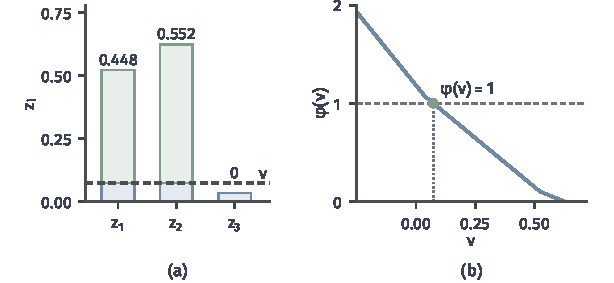
\includegraphics[width=104mm]{figures/05-optimization/06-constrained-optimization/matplotlib/feas-water-level/figure.pdf}
  \caption{单纯形投影的统一阈值，输入$\bm{z}=(0.521875,0.625,0.034375)$。(a)虚线是阈值$\nu$，绿色部分是投影结果，第三个柱子低于阈值，分到$0$。(b)$\varphi(\nu)$是分段线性的递减折线，在每个$z_i$处转折，绿点是$\varphi(\nu)=1$的解$\nu=0.0734375$。}
  \label{fig:feas-water-level}
\end{BookInlineFigure}

\paragraph{求阈值}
把$\bm{z}$从大到小排序为$z_{(1)}\geq\cdots\geq z_{(n)}$。若恰好前$k$个坐标取正，方程~\eqref{eq:feas-simplex-projection}给出
\[
 \nu_k=\frac{1}{k}\Bigl(\sum_{j=1}^kz_{(j)}-1\Bigr).
\]
正确的$k$是满足$z_{(k)}>\nu_k$的最大下标。计算量由排序决定，是$O(n\log n)$。

用图~\ref{fig:feas-water-level}的数据演示。先试$k=3$，$\nu_3=(1.18125-1)/3\approx0.0604$，而最小的坐标$0.034375<0.0604$，不满足要求。再试$k=2$：
\[
 \nu_2=\frac{0.521875+0.625-1}{2}=0.0734375.
\]
这次$z_{(2)}=0.521875>\nu_2$，所以$k=2$，投影是
\[
 \bm{p}=(0.4484375,\;0.5515625,\;0).
\]

\paragraph{投影不是归一化}
把$\bm{z}$除以坐标和也能得到和为一的向量，但这是另一个运算。取$\bm{z}=(0.325,0.625,0.35)$，坐标和$1.3$，归一化得到$(0.25,0.481,0.269)$；投影的阈值是$\nu=0.1$，结果是$(0.225,0.525,0.25)$。投影按相同的量减少各坐标，归一化按相同的比例缩小各坐标。

坐标有负值时差别更大。$\bm{z}'=(0.9,0.5,-0.4)$的坐标和恰好是一，归一化什么也不做，结果仍然不可行。投影取阈值$\nu=0.2$，得到$(0.7,0.3,0)$。图~\ref{fig:feas-projection-cases}(c)在两个坐标的情形画出这种差别：归一化沿过原点的射线回到直线，只有投影沿垂线回来。

\begin{BookInlineFigure}
  \centering
  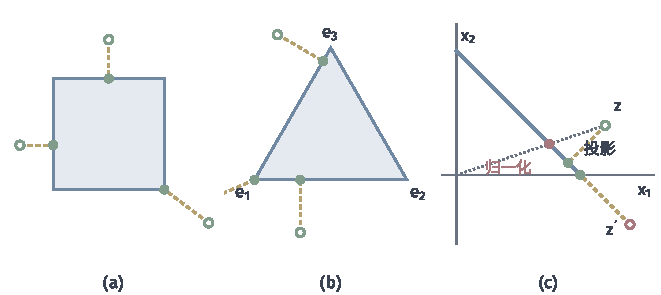
\includegraphics[width=112mm]{figures/05-optimization/06-constrained-optimization/matplotlib/feas-projection-cases/figure.pdf}
  \caption{投影的几何。空心点是输入，实心绿点是投影，黄色虚线是拉回的路径。(a)盒子$[0,1]^2$：逐坐标截断，右下方的点落在角上。(b)单纯形：输入点在三角形所在平面内，可能落到边上，也可能落到顶点。(c)两个坐标的单纯形（蓝线段）：$\bm{z}$的投影与归一化结果（红点，沿过原点的点线）不同；$\bm{z}'$的坐标和已为一，归一化不改变它，它仍然不可行，投影把它送到端点。}
  \label{fig:feas-projection-cases}
\end{BookInlineFigure}

\paragraph{昂贵的投影}
集合复杂时投影没有公式。在$\{\bm{x}:\bm{A}\bm{x}\leq\bm{b}\}$上，式~\eqref{eq:feas-projection}就是一个有$m$个不等式的二次规划，需要用第~\ref{chap:quadratic-conic-programming}章的算法迭代求解。这时外层每一步都包着一个内层优化，内层只能算到有限精度，第~\ref{sec:feas-pgd-step}节会讨论由此带来的误差。

\needspace{6\baselineskip}
\paragraph{变量}
\begin{itemize}
 \item $\bm{x}^{(t)}\in\bm{C}$：当前可行点。
 \item $\bm{g}^{(t)}\in\mathbb{R}^n$：当前梯度。
 \item $\bm{z}^{(t)}\in\mathbb{R}^n$：梯度步的终点，通常不可行。
 \item $\alpha>0$：步长；$\varepsilon>0$与$T$：容差与最大步数。
\end{itemize}

\paragraph{初始化}
取可行起点$\bm{x}^{(0)}\in\bm{C}$，步长$\alpha\leq1/L$，令$t=0$。例中用式~\eqref{eq:feas-running}，取$\alpha=1/L=1/4$，容差$\varepsilon=10^{-3}$，起点和目标值是
\[
 \bm{x}^{(0)}=(0.1,0.2,0.7),\qquad f(\bm{x}^{(0)})=1.25625.
\]

\needspace{6\baselineskip}
\paragraph{每轮更新}
在第$t$轮：
\begin{enumerate}
 \item \textbf{计算梯度步。}令$\bm{z}^{(t)}=\bm{x}^{(t)}-\alpha\bm{g}^{(t)}$。例中第一轮
 \[
  \bm{g}^{(0)}=(-0.9,-1.7,1.4),\qquad \bm{z}^{(0)}=(0.325,0.625,0.35).
 \]
 \item \textbf{投影。}由式~\eqref{eq:feas-simplex-projection}得$\bm{x}^{(t+1)}=P_{\bm{C}}(\bm{z}^{(t)})$。例中第一轮坐标和$1.3$，$k=3$，阈值$\nu=0.1$，于是
 \[
  \bm{x}^{(1)}=(0.225,0.525,0.25),\qquad f(\bm{x}^{(1)})\approx0.38281.
 \]
 \item \textbf{检查停止。}若相邻两点之差的长度除以$\alpha$不超过$\varepsilon$，或$t+1=T$，输出$\bm{x}^{(t+1)}$；否则$t\leftarrow t+1$。例中第一轮这个量约为$2.28$，继续。
\end{enumerate}

例中第二轮，$\bm{g}^{(1)}=(-0.775,-0.4,0.5)$，梯度步终点和投影依次是
\[
 \bm{z}^{(1)}=(0.41875,0.625,0.125),\qquad
 \bm{x}^{(2)}=(0.3625,0.56875,0.06875).
\]
这一轮$\nu=0.05625$，三个坐标仍然为正，$f(\bm{x}^{(2)})\approx0.21426$。

例中第三轮，$\bm{g}^{(2)}=(-0.6375,-0.225,0.1375)$，梯度步终点是图~\ref{fig:feas-water-level}用过的$\bm{z}^{(2)}$。前面已算出$\nu=0.0734375$，第三个坐标被截到零：
\[
 \bm{x}^{(3)}=(0.4484375,0.5515625,0),\qquad f(\bm{x}^{(3)})\approx0.16290.
\]

此后迭代留在底边上。由$x_3=0$和$x_2=1-x_1$代入，每轮的投影化成一维递推
\[
 x_1^{(t+1)}=\tfrac38x_1^{(t)}+\tfrac{5}{16},\qquad t\geq3,
\]
不动点是$x_1=\tfrac12$，误差每轮乘以$\tfrac38$。

第$10$轮的更新量降到容差以下，最终得到$\bm{x}^{(10)}\approx(0.49995,0.50005,0)$。图~\ref{fig:feas-pgd-path}(a)是这条路径，第三步落到活动边之后再也没有离开。

\begin{BookInlineFigure}
  \centering
  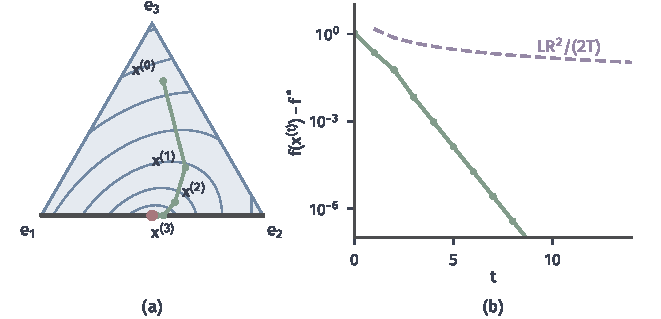
\includegraphics[width=112mm]{figures/05-optimization/06-constrained-optimization/matplotlib/feas-pgd-path/figure.pdf}
  \caption{预算例上的投影梯度法，$\alpha=1/4$，起点$(0.1,0.2,0.7)$。(a)绿色路径在第三步到达活动边（深灰），红点是最优解。(b)绿线是实际目标差，紫色虚线是第~\ref{sec:feas-pgd-step}节证明的上界$LR^2/(2T)$，$R^2=\lVert\bm{x}^{(0)}-\bm{x}^\star\rVert_2^2=0.74$。这个例子强凸，实际收敛比$1/T$快得多。}
  \label{fig:feas-pgd-path}
\end{BookInlineFigure}

\subsection{投影梯度残差}
\label{sec:feas-pgd-residual}

无约束时用$\lVert\nabla f\rVert_2$判断停止。有约束时这把尺子失灵：预算例的最优解处$\nabla f(\bm{x}^\star)=(-\tfrac12,-\tfrac12,0)$并不为零。那么应该用什么量来判断“已经到了”？

\paragraph{残差的定义}
一个点走不动，意思是走一步再投影又回到原地。把这个位移除以步长，单位就和梯度一致。

\begin{definition}[投影梯度残差]
\label{def:feas-residual}
设$\alpha>0$，$\bm{x}\in\bm{C}$。称
\begin{equation}
 \bm{G}_\alpha(\bm{x})=\frac{1}{\alpha}\Bigl[\bm{x}-P_{\bm{C}}\bigl(\bm{x}-\alpha\nabla f(\bm{x})\bigr)\Bigr]
 \label{eq:feas-residual}
\end{equation}
为\term{投影梯度残差}（projected gradient residual）。
\end{definition}

$\bm{C}=\mathbb{R}^n$时投影不起作用，$\bm{G}_\alpha=\nabla f$，所以它是梯度的推广。第~\ref{sec:feas-pgd-projection}节的停止量正是$\lVert\bm{G}_\alpha(\bm{x}^{(t)})\rVert_2$。

\paragraph{残差为零意味着什么}
凸集上的一阶必要条件是下面的\term{变分不等式}（variational inequality）：对可行方向$\bm{y}-\bm{x}$，目标的方向导数不能为负。推导很短：若$\bm{x}$是局部极小点，$\bm{y}\in\bm{C}$，线段$\bm{x}+s(\bm{y}-\bm{x})$在$s\in[0,1]$上可行，所以
\[
 0\leq\lim_{s\downarrow0}\frac{f(\bm{x}+s(\bm{y}-\bm{x}))-f(\bm{x})}{s}=\langle\nabla f(\bm{x}),\bm{y}-\bm{x}\rangle.
\]

\begin{theorem}[残差为零与变分不等式]
\label{thm:feas-residual}
设$\bm{C}$非空闭凸，$f$在$\bm{x}\in\bm{C}$处可微，$\alpha>0$。则$\bm{G}_\alpha(\bm{x})=\bm{0}$当且仅当
\begin{equation}
 \langle\nabla f(\bm{x}),\bm{y}-\bm{x}\rangle\geq0,\quad\forall\bm{y}\in\bm{C}.
 \label{eq:feas-vi}
\end{equation}
若$f$还是凸函数，这又等价于$\bm{x}$是$f$在$\bm{C}$上的全局最优解。
\end{theorem}

\begin{proof}
$\bm{G}_\alpha(\bm{x})=\bm{0}$就是$\bm{x}=P_{\bm{C}}(\bm{x}-\alpha\nabla f(\bm{x}))$。在式~\eqref{eq:feas-projection-vi}中取$\bm{p}=\bm{x}$，$\bm{z}=\bm{x}-\alpha\nabla f(\bm{x})$，这等价于
\[
 \langle-\alpha\nabla f(\bm{x}),\bm{y}-\bm{x}\rangle\leq0,\quad\forall\bm{y}\in\bm{C}.
\]
除以$-\alpha<0$，不等号反向，即得式~\eqref{eq:feas-vi}。

$f$凸时，切平面从下方托住目标，所以
\[
 f(\bm{y})\geq f(\bm{x})+\langle\nabla f(\bm{x}),\bm{y}-\bm{x}\rangle\geq f(\bm{x}),
\]
$\bm{x}$是全局最优解。反方向是前面的一阶必要条件。
\end{proof}

条件~\eqref{eq:feas-vi}里没有$\alpha$，所以残差对某一个$\alpha$为零，就对所有$\alpha>0$为零。残差的大小则随$\alpha$变化，比较时要固定步长。

\paragraph{边界最优点}
现在验证预算例的解。在$\bm{x}^\star=(\tfrac12,\tfrac12,0)$处，对任意$\bm{y}\in\bm{\Delta}$，利用$y_1+y_2=1-y_3$，得到
\[
 \langle\nabla f(\bm{x}^\star),\bm{y}-\bm{x}^\star\rangle
 =-\tfrac12(y_1+y_2)+\tfrac12
 =\tfrac12y_3\geq0.
\]
变分不等式成立，目标凸，所以$\bm{x}^\star$是全局最优解。把它代入式~\eqref{eq:feas-running}，得到
\[
 f^\star=\tfrac12\bigl[\tfrac14+\tfrac{1}{16}\bigr]=\tfrac{5}{32}.
\]

梯度不为零，但它指向的是“出不去”的方向。这就好比一个人靠墙站着，墙外地势更低：坡度不为零，他却走不动。图~\ref{fig:feas-boundary-residual}对比了两个边界点。最优点的梯度步终点垂直于活动边，投影原路拉回。另一个点的梯度步有沿边的分量，投影之后确实前进了。

\begin{BookInlineFigure}
  \centering
  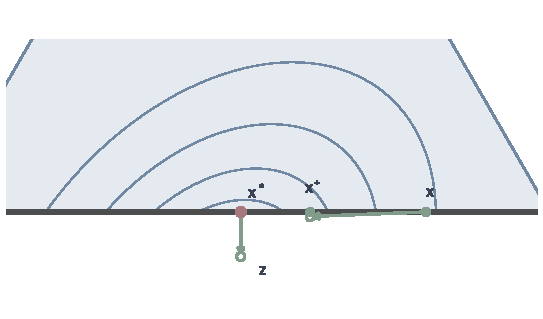
\includegraphics[width=92mm]{figures/05-optimization/06-constrained-optimization/matplotlib/feas-boundary-residual/figure.pdf}
  \caption{残差在活动边上的含义，局部放大底边，$\alpha=1/4$。红点$\bm{x}^\star$处，平面内的梯度步（绿色箭头）垂直离开边，投影回到原处，残差为零而梯度不为零。右侧的$\bm{x}=(0.2,0.8,0)$处，梯度步有沿边分量，投影后到达$\bm{x}^{+}$，残差不为零。}
  \label{fig:feas-boundary-residual}
\end{BookInlineFigure}

\paragraph{非凸时残差只检验驻定}
定理~\ref{thm:feas-residual}的后半句依赖凸性。取一元函数$f(x)=-x^2$，$\bm{C}=[-1,2]$。残差为零的点有三个：$x=-1$、$x=0$、$x=2$。

图~\ref{fig:feas-nonconvex-residual}画出了它们。$x=0$是目标的局部极大点；$x=-1$是约束上的局部极小点，$f=-1$；只有$x=2$是全局最优解，$f=-4$。残差只说明“在一阶意义下走不动”，不区分这三种情况。

\begin{BookInlineFigure}
  \centering
  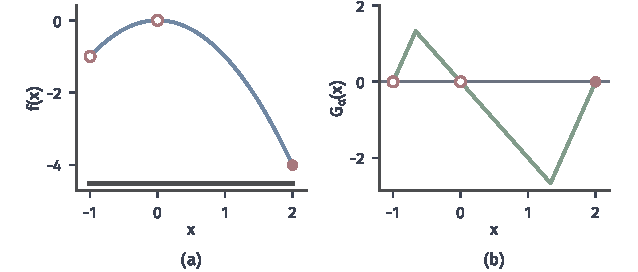
\includegraphics[width=108mm]{figures/05-optimization/06-constrained-optimization/matplotlib/feas-nonconvex-residual/figure.pdf}
  \caption{非凸目标$f(x)=-x^2$，$\bm{C}=[-1,2]$（深灰线）。(a)目标曲线，空心红点是局部极大点$0$和局部极小点$-1$，实心红点是全局最优解$2$。(b)$\alpha=1/4$时的残差$G_\alpha(x)$，在这三个点上都为零。}
  \label{fig:feas-nonconvex-residual}
\end{BookInlineFigure}

\subsection{步长与误差}
\label{sec:feas-pgd-step}

残差为零是目标。迭代是否真的把残差推向零，又需要什么步长？投影只能近似时，保证还剩多少？

\paragraph{单步下降}
投影性质~\eqref{eq:feas-projection-vi}告诉我们投影后的位移仍然是一个下降方向，这是下面所有结论的基础。

\begin{theorem}[投影梯度的单步下降]
\label{thm:feas-pgd-descent}
设$\bm{C}$非空闭凸，$f$在包含$\bm{C}$的开集上可微，且在$\bm{C}$上$L$光滑。对$\bm{x}\in\bm{C}$和$\alpha>0$，记$\bm{x}^{+}$是式~\eqref{eq:feas-pgd}的新点，有
\begin{equation}
 f(\bm{x}^{+})\leq f(\bm{x})-\alpha\Bigl(1-\frac{L\alpha}{2}\Bigr)\lVert\bm{G}_\alpha(\bm{x})\rVert_2^2.
 \label{eq:feas-pgd-descent}
\end{equation}
\end{theorem}

\begin{proof}
在式~\eqref{eq:feas-projection-vi}中取$\bm{z}=\bm{x}-\alpha\nabla f(\bm{x})$，$\bm{p}=\bm{x}^{+}$，$\bm{y}=\bm{x}$，得到
\[
 \langle\bm{x}-\alpha\nabla f(\bm{x})-\bm{x}^{+},\bm{x}-\bm{x}^{+}\rangle\leq0.
\]

整理后得到投影位移与梯度的内积：
\[
 \langle\nabla f(\bm{x}),\bm{x}^{+}-\bm{x}\rangle\leq-\frac1\alpha\lVert\bm{x}^{+}-\bm{x}\rVert_2^2.
\]

$\bm{C}$凸，线段$[\bm{x},\bm{x}^{+}]$在$\bm{C}$中，下降引理可用，于是
\[
 f(\bm{x}^{+})\leq f(\bm{x})+\langle\nabla f(\bm{x}),\bm{x}^{+}-\bm{x}\rangle+\frac L2\lVert\bm{x}^{+}-\bm{x}\rVert_2^2.
\]

把前一式代入，再用$\bm{x}^{+}-\bm{x}=-\alpha\bm{G}_\alpha(\bm{x})$，即得式~\eqref{eq:feas-pgd-descent}。
\end{proof}

只要$0<\alpha<2/L$，式~\eqref{eq:feas-pgd-descent}的括号就是正的，目标严格下降，除非已经驻定。这和无约束的下降估计形式完全相同，只是把梯度换成了残差。

\paragraph{非凸问题}
目标非凸时目标差无从谈起，能评价的是残差。这里需要目标在集合上有下界，否则下降可以无休止地进行。

\begin{theorem}[非凸情形的投影梯度]
\label{thm:feas-pgd-nonconvex}
在定理~\ref{thm:feas-pgd-descent}的条件下，设$f_{\inf}=\inf_{\bm{C}}f>-\infty$，取$\alpha=1/L$，则对$T\geq1$，
\begin{equation}
 \min_{0\leq t<T}\lVert\bm{G}_\alpha(\bm{x}^{(t)})\rVert_2^2\leq\frac{2L\bigl(f(\bm{x}^{(0)})-f_{\inf}\bigr)}{T},
 \label{eq:feas-pgd-nonconvex}
\end{equation}
并且$\{\bm{x}^{(t)}\}$的每个极限点都满足变分不等式~\eqref{eq:feas-vi}。
\end{theorem}

\begin{proof}
由式~\eqref{eq:feas-pgd-descent}，$\alpha=1/L$时
\[
 \frac{1}{2L}\lVert\bm{G}_\alpha(\bm{x}^{(t)})\rVert_2^2\leq f(\bm{x}^{(t)})-f(\bm{x}^{(t+1)}).
\]
对$t=0,\ldots,T-1$求和，右端裂项，并用$f(\bm{x}^{(T)})\geq f_{\inf}$，最小值不超过平均值，即得式~\eqref{eq:feas-pgd-nonconvex}。

级数$\sum_t\lVert\bm{G}_\alpha(\bm{x}^{(t)})\rVert_2^2$收敛，所以残差趋于零。若梯度连续，投影非扩张保证$\bm{G}_\alpha$连续，极限点处残差为零。定理~\ref{thm:feas-residual}给出结论。
\end{proof}

\paragraph{凸问题}
加上凸性和解的存在，可以用目标差衡量。证明的关键是把一步的目标差写成到解距离平方的差，这样求和时能够裂项。

\begin{theorem}[凸情形的投影梯度]
\label{thm:feas-pgd-convex}
在定理~\ref{thm:feas-pgd-descent}的条件下，设$f$在$\bm{C}$上凸，且存在最优解$\bm{x}^\star\in\bm{C}$，取$\alpha=1/L$。则对$T\geq1$，
\begin{equation}
 f(\bm{x}^{(T)})-f^\star\leq\frac{L\lVert\bm{x}^{(0)}-\bm{x}^\star\rVert_2^2}{2T}.
 \label{eq:feas-pgd-convex}
\end{equation}
若$f$还在$\bm{C}$上$\mu$强凸，$\mu>0$，则
\begin{equation}
 \lVert\bm{x}^{(t+1)}-\bm{x}^\star\rVert_2^2\leq\Bigl(1-\frac\mu L\Bigr)\lVert\bm{x}^{(t)}-\bm{x}^\star\rVert_2^2.
 \label{eq:feas-pgd-strong}
\end{equation}
\end{theorem}

\begin{proof}
记$\bm{x}=\bm{x}^{(t)}$，$\bm{x}^{+}=\bm{x}^{(t+1)}$，$\bm{g}=\nabla f(\bm{x})$，$\bm{y}\in\bm{C}$任取。由下降引理和$\mu$强凸的下界（$\mu=0$即凸），得到
\[
 \begin{aligned}
 f(\bm{x}^{+})&\leq f(\bm{x})+\langle\bm{g},\bm{x}^{+}-\bm{x}\rangle+\frac L2\lVert\bm{x}^{+}-\bm{x}\rVert_2^2,\\
 f(\bm{y})&\geq f(\bm{x})+\langle\bm{g},\bm{y}-\bm{x}\rangle+\frac\mu2\lVert\bm{y}-\bm{x}\rVert_2^2.
 \end{aligned}
\]

两式相减，消去$f(\bm{x})$：
\[
 f(\bm{x}^{+})-f(\bm{y})\leq\langle\bm{g},\bm{x}^{+}-\bm{y}\rangle+\frac L2\lVert\bm{x}^{+}-\bm{x}\rVert_2^2-\frac\mu2\lVert\bm{y}-\bm{x}\rVert_2^2.
\]

在式~\eqref{eq:feas-projection-vi}中取$\bm{z}=\bm{x}-\bm{g}/L$，$\bm{p}=\bm{x}^{+}$，整理得
\[
 \langle\bm{g},\bm{x}^{+}-\bm{y}\rangle\leq L\langle\bm{x}-\bm{x}^{+},\bm{x}^{+}-\bm{y}\rangle.
\]

再用恒等式展开$\lVert\bm{x}-\bm{y}\rVert_2^2$，它把内积化成三个距离平方：
\[
 2\langle\bm{x}-\bm{x}^{+},\bm{x}^{+}-\bm{y}\rangle
 =\lVert\bm{x}-\bm{y}\rVert_2^2-\lVert\bm{x}-\bm{x}^{+}\rVert_2^2-\lVert\bm{x}^{+}-\bm{y}\rVert_2^2.
\]

代回去，$\lVert\bm{x}^{+}-\bm{x}\rVert_2^2$的项抵消，得到
\[
 f(\bm{x}^{+})-f(\bm{y})\leq\frac{L-\mu}{2}\lVert\bm{x}-\bm{y}\rVert_2^2-\frac L2\lVert\bm{x}^{+}-\bm{y}\rVert_2^2.
\]

取$\bm{y}=\bm{x}^\star$，左端非负，移项除以$L/2$，就是式~\eqref{eq:feas-pgd-strong}；$\mu=0$时说明到解的距离不增。

$\mu=0$时对$t=0,\ldots,T-1$求和，右端裂项：
\[
 \sum_{t=1}^T\bigl(f(\bm{x}^{(t)})-f^\star\bigr)\leq\frac L2\lVert\bm{x}^{(0)}-\bm{x}^\star\rVert_2^2.
\]
由定理~\ref{thm:feas-pgd-descent}目标逐步下降，最后一项最小，不超过平均值，即得式~\eqref{eq:feas-pgd-convex}。
\end{proof}

预算例中$R^2=0.74$，$L=4$，上界是$1.48/T$，$T=1$时为$1.48$，实际目标差是$0.2266$。强凸的保证给出距离平方每步至少乘以$\tfrac34$。实际到达活动边之后因子是$(\tfrac38)^2\approx0.14$。约束把自由度减到一维，沿边方向$(1,-1,0)$的曲率是$\tfrac52$，比全空间最小的曲率$\mu=1$大。

\paragraph{$L$未知时}
可以用回溯代替固定步长：试探$\alpha$，算出$\bm{x}^{+}$，检查
\[
 f(\bm{x}^{+})\leq f(\bm{x})+\langle\nabla f(\bm{x}),\bm{x}^{+}-\bm{x}\rangle+\frac{1}{2\alpha}\lVert\bm{x}^{+}-\bm{x}\rVert_2^2,
\]
不满足就缩短$\alpha$。上面的证明只用到这个不等式，结论把$L$换成$1/\alpha_{\min}$仍成立。要注意，换一次$\alpha$就要重新投影，集合复杂时这是真实的成本。

\paragraph{近似投影}
投影由内层迭代求出时，输出$\tilde{\bm{x}}^{+}$与真投影有差距。设
\[
 \bigl\lVert\tilde{\bm{x}}^{+}-P_{\bm{C}}(\bm{x}-\alpha\nabla f(\bm{x}))\bigr\rVert_2\leq\varepsilon_t.
\]
这个误差有三种影响，要分别看待。

第一是可行性。输出到$\bm{C}$的距离不超过$\varepsilon_t$，但不一定是零，所以要单独检查原约束的残差。

第二是误差传播。设$f$的光滑、强凸条件在含所有迭代点的凸集上成立，定理~\ref{thm:feas-pgd-convex}说明精确映射把到解的距离至少缩小到$\rho=\sqrt{1-\mu/L}$倍。再加上三角不等式，得到
\begin{equation}
 \lVert\bm{x}^{(t+1)}-\bm{x}^\star\rVert_2\leq\rho\lVert\bm{x}^{(t)}-\bm{x}^\star\rVert_2+\varepsilon_t.
 \label{eq:feas-inexact-recursion}
\end{equation}

$\varepsilon_t\equiv\varepsilon$时展开递推，几何级数求和，距离的上极限不超过$\varepsilon/(1-\rho)$，迭代停在一个与内层精度成比例的范围里。没有强凸时$\rho=1$，上界只能写成$\lVert\bm{x}^{(0)}-\bm{x}^\star\rVert_2+\sum_t\varepsilon_t$，误差必须可求和才不累积。

第三是残差本身。用近似投影算出的残差$\tilde{\bm{G}}_\alpha$满足
\[
 \bigl\lvert\lVert\tilde{\bm{G}}_\alpha\rVert_2-\lVert\bm{G}_\alpha\rVert_2\bigr\rvert\leq\frac{\varepsilon_t}{\alpha}.
\]
所以步长越小，停止量受内层误差的污染越重。图~\ref{fig:feas-inexact-projection}显示了前两种影响。预算例中$\rho\approx0.866$，$1/(1-\rho)\approx7.46$。

\begin{BookInlineFigure}
  \centering
  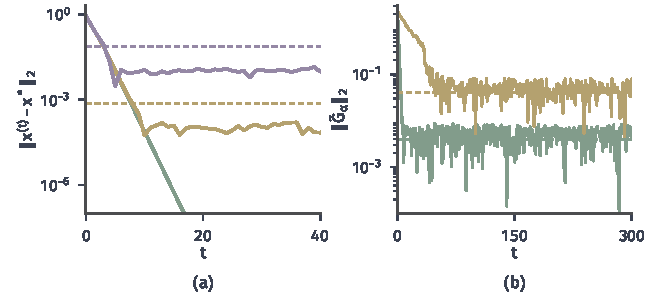
\includegraphics[width=112mm]{figures/05-optimization/06-constrained-optimization/matplotlib/feas-inexact-projection/figure.pdf}
  \caption{近似投影的影响，在每次投影结果上叠加固定种子的随机扰动，长度为$\varepsilon$。(a)到解的距离：绿线是精确投影，黄线$\varepsilon=10^{-4}$，紫线$\varepsilon=10^{-2}$，同色虚线是上界$\varepsilon/(1-\rho)$；距离停在上界之内。(b)$\varepsilon=10^{-3}$时算出的残差：绿线$\alpha=1/4$，黄线$\alpha=1/40$，同色虚线是$\varepsilon/\alpha$；步长小，平台反而高。}
  \label{fig:feas-inexact-projection}
\end{BookInlineFigure}

\paragraph{接近可行不等于接近最优}
内层把“输出离集合多远”算得很准，不能说明外层接近了解。预算例的顶点$\bm{e}_2=(0,1,0)$完全可行，可行误差为零，它的目标差却是$0.625$。可行性和最优性是两件事，都要报告。
